% !TEX root = main.tex
\documentclass[11pt, a4paper]{report}

% ------------------------------------------------------------------------------
% Page Geometry & Margins
% ------------------------------------------------------------------------------
\usepackage[
    top=1.0in,
    bottom=1.0in,
    left=1.0in,
    right=1.0in,
    headheight=14.5pt,
    headsep=0.35in,
    footskip=0.4in
]{geometry}

% ------------------------------------------------------------------------------
% Typography & Fonts
% ------------------------------------------------------------------------------
\usepackage{mathptmx} % Times Roman style typography
\usepackage[utf8]{inputenc}
\usepackage[T1]{fontenc}
\usepackage{microtype}

% ------------------------------------------------------------------------------
% Math & Symbols
% ------------------------------------------------------------------------------
\usepackage{amsmath, amsfonts, amssymb}

% ------------------------------------------------------------------------------
% Tables, Lists & Visual Boxes
% ------------------------------------------------------------------------------
\usepackage{booktabs}
\usepackage{tabularx}
\usepackage{enumitem}
\usepackage{graphicx}
\usepackage{xcolor}
\usepackage{tcolorbox}

% ------------------------------------------------------------------------------
% Headers & Footers
% ------------------------------------------------------------------------------
\usepackage{fancyhdr}
\pagestyle{fancy}
\fancyhf{}
\fancyhead[L]{\small\slshape Electronics Engineering Learning Module}
\fancyhead[R]{\small\slshape\nouppercase{\leftmark}}
\fancyfoot[C]{\thepage}
\renewcommand{\headrulewidth}{0.4pt}
\renewcommand{\footrulewidth}{0pt}

\fancypagestyle{plain}{
    \fancyhf{}
    \fancyfoot[C]{\thepage}
    \renewcommand{\headrulewidth}{0pt}
}

% ------------------------------------------------------------------------------
% Hyperlinks & Bibliography
% ------------------------------------------------------------------------------
\usepackage{cite}
\usepackage{hyperref}
\hypersetup{
    colorlinks=true,
    linkcolor=blue!70!black,
    citecolor=green!50!black,
    urlcolor=blue!80!black
}

% ------------------------------------------------------------------------------
% Custom Boxes & Placeholders
% ------------------------------------------------------------------------------
\newtcolorbox{safetybox}[1][]{
    colback=red!5!white,
    colframe=red!75!black,
    fonttitle=\bfseries,
    title=Laboratory Safety Notice,
    #1
}

\newtcolorbox{activitybox}[1][]{
    colback=blue!5!white,
    colframe=blue!75!black,
    fonttitle=\bfseries,
    title=Hands-On Lab Activity Protocol,
    #1
}

\newcommand{\imageplaceholder}[3][3.5cm]{
    \begin{figure}[htbp]
        \centering
        \begin{tcolorbox}[
            colback=gray!8!white,
            colframe=gray!50!black,
            width=0.92\textwidth,
            halign=center
        ]
            \vspace{0.2cm}
            \textbf{\Large [ Figure: #2 ]} \\[0.4em]
            \textit{Suggested asset file: \texttt{figures/\detokenize{#3}}} \\[0.3em]
            \small (Image omitted per user specification; drop the graphic file in \texttt{figures/} and substitute with \texttt{\textbackslash includegraphics} when available.)
            \vspace{0.2cm}
        \end{tcolorbox}
        \caption{#2}
        \label{fig:\detokenize{#3}}
    \end{figure}
}
% ------------------------------------------------------------------------------
% Document Metadata
% ------------------------------------------------------------------------------
\title{
    \vspace{-1.5cm}
    \textbf{\Huge Electronics Workshop Module}
}
\author{\textbf{Ateneo Computer Engineering Society}}
\date{Academic Year 2026--2027}

% ------------------------------------------------------------------------------
% Document Body
% ------------------------------------------------------------------------------
\begin{document}

\maketitle

\begin{abstract}
This laboratory training module serves as a rigorous, practical curriculum designed to equip engineering students and technicians with essential competencies in laboratory safety standards, occupational hazard compliance, component characterization, solderless breadboard prototyping, systematic circuit troubleshooting, and foundational soldering techniques. By pairing standard safety protocols with structured hands-on procedures and diagnostic methodologies, this manual prepares students for safe, effective experimentation in advanced electronics coursework and practical laboratory environments.
\end{abstract}

\vspace{1em}
\section*{Module Objectives \& Competencies}
Upon successful completion of this exhaustive learning module, students and technical trainees will be able to demonstrate mastery across the following domain competencies:
\begin{itemize}[leftmargin=1.5em]
    \item \textbf{Practice Laboratory Safety:} Identify hazard types, physiological shock thresholds, PPE, bench housekeeping, and emergency protocols in electronics labs \cite{yildiz2010approach, bicol_university_safety}.
    \item \textbf{Identify \& Characterize Basic Components:} Distinguish passive and active devices including resistors, capacitors, inductors, diodes, LEDs, transistors, and integrated circuits \cite{seymour_components, kalyanaraman_circuits}.
    \item \textbf{Build \& Prototype Circuits:} Interpret schematic diagrams and construct working prototypes on standard solderless breadboards \cite{sparkfun_breadboard}.
    \item \textbf{Troubleshoot \& Diagnose Faults:} Systematically isolate circuit anomalies using point-to-point node voltage tracing and continuity analysis.
    \item \textbf{Execute Reliable Soldering:} Form high-integrity electrical solder joints, perform tip maintenance, and diagnose defective connections.
\end{itemize}

\section*{Prerequisites \& Required Materials}
\begin{itemize}[leftmargin=1.5em]
    \item Basic familiarity with introductory algebra and physics coursework topics.
    \item Laptop or tablet with internet access and engineering tools.
    \item Standard lab inventory: Breadboard kit, jumper wires, DMM, variable DC power supply, components (resistors, LEDs, transistors), and soldering iron station.
\end{itemize}

\tableofcontents
\newpage

% ------------------------------------------------------------------------------
% Modular Chapters
% ------------------------------------------------------------------------------
% !TEX root = ../main.tex
\chapter{Laboratory Safety Protocols}

\section{Electrical Hazards \& Human Physiology}
Electronics laboratory environments present personnel with hazardous voltages, arc flash hazards, thermal sources, toxic chemical vapors during soldering, and sensitive electrostatic discharge (ESD) risks. Compliance with occupational health and safety standards \cite{yildiz2010approach, bicol_university_safety} is essential to maintain a zero-injury environment.

\subsection{Current vs. Voltage: Physiological Impact}
A primary tenet of electrical safety is that \textbf{electric current}, rather than voltage alone, determines physiological trauma. The human body behaves as an electrolytic volume conductor whose internal impedance varies drastically depending on tissue hydration, contact surface area, and skin moisture.

These physiological thresholds were empirically quantified through the landmark biomedical research of Professor Charles F. Dalziel at the University of California, Berkeley \cite{dalziel1968lethal}. Dalziel's extensive experimental trials on human sensory perception and muscular tetany established the definitive criteria for current tolerance across commercial power frequencies ($50\text{--}60\text{ Hz}$). His findings subsequently served as the foundational basis for international regulatory standards, including the International Electrotechnical Commission Technical Report \textbf{IEC TR 60479-1} \cite{iec60479_1}, \textbf{OSHA Publication 3075} (\textit{Controlling Electrical Hazards}) \cite{osha3075}, and \textbf{IEEE Standard 80} \cite{ieee80}.

\begin{table}[htbp]
    \centering
    \caption{Physiological Effects of 60 Hz Alternating Current on the Human Body}
    \label{tab:shock_thresholds}
    \begin{tabularx}{\textwidth}{p{2.8cm} p{4.2cm} X}
        \toprule
        \textbf{Current Level} & \textbf{Threshold Name} & \textbf{Physiological Reaction} \\
        \midrule
        $1\text{ mA}$ ($0.001\text{ A}$) & Perception Threshold & Faint tingling sensation at contact point; generally harmless. \\
        $10\text{ mA}$ ($0.010\text{ A}$) & ``Let-Go'' Threshold & Involuntary muscle contraction; motor control lost; victim cannot release energized conductor. \\
        $20\text{--}30\text{ mA}$ & Respiratory Paralysis & Severe thoracic muscle tetany; breathing arrests; rapid asphyxiation if loop is sustained. \\
        $\ge 100\text{ mA}$ ($0.1\text{ A}$) & Ventricular Fibrillation & Uncoordinated cardiac twitching; blood circulation ceases; fatal within seconds if not defibrillated. \\
        \midrule
        \multicolumn{3}{l}{\footnotesize\textit{Sources: Dalziel \& Lee (IEEE) \cite{dalziel1968lethal}, IEC TR 60479-1 \cite{iec60479_1}, and OSHA Pub.~3075 \cite{osha3075}.}} \\
        \bottomrule
    \end{tabularx}
\end{table}
\subsection{Body Resistance \& Environmental Variables}
Intact, calloused dry skin offers a resistance between $100\text{ k}\Omega$ and $500\text{ k}\Omega$. However, when skin is broken, punctured, or saturated with perspiration, skin resistance collapses below $1\text{ k}\Omega$. Under wet conditions, voltages as low as \textbf{50 V} can deliver lethal currents exceeding $50\text{ mA}$ across the chest. Furthermore, high-voltage test equipment (such as cathode ray tubes or inductive supplies) can exceed $10{,}000\text{ V}$, making liquid spills an immediate life hazard.

\begin{safetybox}
\textbf{CRITICAL SAFETY RULES FOR THE BENCH:}
\begin{itemize}[leftmargin=1.2em]
    \item \textbf{Remove All Conductive Jewelry:} Metallic rings, bracelets, watches, and chains drastically lower skin contact resistance and can cause severe flash burns or direct shock paths.
    \item \textbf{The ``One-Hand Rule'':} When probing circuits with potentially dangerous potentials, keep your non-dominant hand in a pocket or behind your back. This prevents forming a closed circuit loop across both arms through the thoracic cavity and heart.
    \item \textbf{No Food or Beverages:} Drinks near workbenches are strictly prohibited to prevent conductive fluid spills into energized test instruments.
    \item \textbf{Verify Zero Potential:} Treat all circuits as energized until de-energizing and physically verifying zero potential with a calibrated Digital Multimeter (DMM).
\end{itemize}
\end{safetybox}

\section{Facility Safety, Grounding, \& Fire Protection}
Workstations must utilize three-prong grounded power distribution equipped with Ground Fault Circuit Interrupters (GFCIs) or isolation transformers for AC power line equipment. Workstations must maintain clear access to:
\begin{itemize}[leftmargin=1.5em]
    \item Emergency master power disconnect shutoffs.
    \item Class C or Class ABC dry chemical/CO$_2$ fire extinguishers rated for energized electrical equipment. Never apply water to an electrical fire.
    \item Standard first aid stations and eye-wash facilities.
\end{itemize}

\section{Electrostatic Discharge (ESD) Prevention}
Friction from clothing and walking across polymer flooring can generate static charges exceeding \textbf{5,000 V}. Human sensory perception detects static discharges only above 3,500--4,000 V, yet fragile semiconductor junction gates (especially MOSFETs) can suffer dielectric breakdown from pulses as low as 20--50 V.

Technicians must wear grounded anti-static wrist straps incorporating a minimum $500\text{ k}\Omega$ (standard $1\text{ M}\Omega$) safety series resistor. This resistor safely drains electrostatic accumulation to earth ground while providing adequate impedance to limit current to safe sub-milliampere levels in case the operator touches an energized mains conductor.

\section{Workbench Housekeeping \& Shutdown Protocol}
At the end of every laboratory session, technicians must transition the bench into ``Secure Mode'':
\begin{enumerate}[leftmargin=1.5em]
    \item Power down all signal generators, oscilloscopes, and DC power supplies.
    \item Reset variable voltage and current knobs to zero.
    \item Clean and tin soldering iron tips, confirm irons are seated in insulated stands, and turn off iron mains power.
    \item Return passive components to sorted bin cabinets and store leads and tools in labeled drawers.
\end{enumerate}

\section{Laboratory Power Tool Operation \& Mechanical Safety}
Power tools commonly utilized in electronics laboratories---such as benchtop PCB drill presses, rotary cutting tools, and hot air rework stations---introduce severe mechanical and thermal hazards alongside electrical risks. Safe operation requires strict adherence to mechanical protocols:

\begin{itemize}[leftmargin=1.5em]
    \item \textbf{Workpiece Clamping:} Never hold a printed circuit board or chassis enclosure by hand during drilling or cutting operations. The rotational torque of high-speed bits can snatch the workpiece, causing violent projectile ejection or deep lacerations. Workpieces must always be immobilized using a mechanical drill press vise or PCB fixture.
    \item \textbf{Entanglement Prevention \& Dress Code:} Rotating spindles present an immediate entanglement hazard. Personnel must strictly observe a \textbf{zero-gloves rule} when operating drills and rotary tools, as fabric can become ensnared in spinning chucks. Long hair must be tied back securely, long sleeves rolled above the elbows, and lanyards, loose jewelry, and neckties removed prior to operating machinery.
    \item \textbf{Particulate and Eye Protection:} Machining copper-clad FR4 (flame-retardant fiberglass epoxy) generates microscopic glass dust and sharp copper burrs. Operators must wear ANSI Z87.1-rated safety glasses with side shields and an N95 particulate respirator to prevent corneal abrasion and inhalation of toxic fiberglass particulates.
    \item \textbf{Tool Maintenance \& Disconnection:} Always disconnect power from rotary tools and drill presses before changing drill bits, cutting discs, or sanding drums. Never leave an energized tool unattended on a workbench.
\end{itemize}

\section{PCB Etchant Chemical Safety: Storage, Neutralization \& Disposal}
Wet chemical etching processes commonly employ acidic oxidizers such as Ferric Chloride ($\text{FeCl}_3$) or Ammonium/Sodium Persulfate to dissolve unwanted copper laminate. Because these solutions are highly corrosive and toxic, handling them demands strict compliance with occupational safety and environmental regulations:

\subsection{Storage Protocols}
\begin{itemize}[leftmargin=1.5em]
    \item \textbf{Chemical Compatibility:} Ferric chloride and persulfate solutions must be stored strictly in acid-resistant, heavy-duty High-Density Polyethylene (HDPE), polypropylene, or fluoropolymer containers with hermetic seals. \textbf{Never store or mix etchants in metallic containers or sinks}, as the acid reacts vigorously with metals, generating corrosive fumes and risking container rupture.
    \item \textbf{Environment and Segregation:} Store etchant bottles inside a dedicated, ventilated acid/corrosive chemical cabinet. Keep containers isolated from organic solvents, flammable materials, strong bases (which cause exothermic reactions), and direct ultraviolet sunlight.
    \item \textbf{Container Labeling:} Every container must bear GHS-compliant hazardous labeling clearly stating the chemical name, concentration, preparation date, and specific hazard warnings (Corrosive, Environmental Hazard).
\end{itemize}

\subsection{Neutralization and Disposal Protocols}
\begin{itemize}[leftmargin=1.5em]
    \item \textbf{Strict Prohibition of Drain Disposal:} \textbf{Spent etchant solutions must NEVER be poured into domestic, commercial, or municipal plumbing.} Dissolved cupric ions ($\text{Cu}^{2+}$) are highly biocidal, permanently disrupt biological wastewater treatment facilities, and rapidly dissolve copper and steel drainage piping.
    \item \textbf{Pre-Disposal Neutralization:} Before transfer, spent acidic etchant must be slowly neutralized by gradually adding a weak base such as Sodium Bicarbonate (baking soda, $\text{NaHCO}_3$) or Calcium Carbonate ($\text{CaCO}_3$) in a well-ventilated fume hood until carbon dioxide effervescence ceases ($\text{pH} \approx 7.0\text{--}8.0$). This reaction converts toxic soluble copper ions into insoluble copper carbonate/hydroxide precipitate.
    \item \textbf{Collection and Institutional Hand-off:} Allow the precipitated copper sludge to settle. Decant the neutral liquid and collect the sludge in designated hazardous chemical waste carboys labeled ``Spent Copper Etchant Sludge''. Submit containers to the University Environmental Safety Office or a licensed hazardous chemical disposal contractor in full compliance with local environmental legislation (e.g., DENR standards).
\end{itemize}

% !TEX root = ../main.tex
\chapter{Basic Electronic Components \& Circuit Fundamentals}

\section{Taxonomy of Electronic Components}
Electronic components are the foundational physical building blocks of all electrical networks \cite{seymour_components, kalyanaraman_circuits}. Components are broadly classified by their energetic behavior into \textbf{passive} and \textbf{active} devices:

\begin{itemize}[leftmargin=1.5em]
    \item \textbf{Passive Components:} Devices that cannot deliver net power gain or inject external energy into a network. They dissipate, store, or release energy present in the circuit.
    \item \textbf{Active Components:} Devices that rely on an external power source to amplify electrical signals, control directional power flow, or provide electronic switching.
\end{itemize}

\section{Fundamental Passive Components}

\subsection{Resistors}
Resistors introduce precise electrical opposition to electric current, functioning to divide voltages, limit branch currents, and set active component bias operating points \cite{seymour_components}. Standard axial-lead resistors are fabricated using carbon film or metal film compositions, with values marked by standardized 4-band or 5-band color codes.

As current flows through a resistor, electrical energy is converted into thermal energy ($P = I^2 R = V \cdot I$). Consequently, resistors are categorized by their continuous physical power dissipation ratings:
\begin{itemize}[leftmargin=1.5em]
    \item \textbf{Standard Signal Resistors ($1/4\text{ W}$ and $1/2\text{ W}$):} Small cylindrical packages suitable for breadboard prototyping and low-power control lines.
    \item \textbf{Power Resistors ($1\text{ W}$ to $5\text{ W}+$):} Larger bodies, often encapsulated in white rectangular ceramic cement blocks, designed for power supplies and motor drivers.
\end{itemize}

\begin{figure}[htbp]
    \centering
    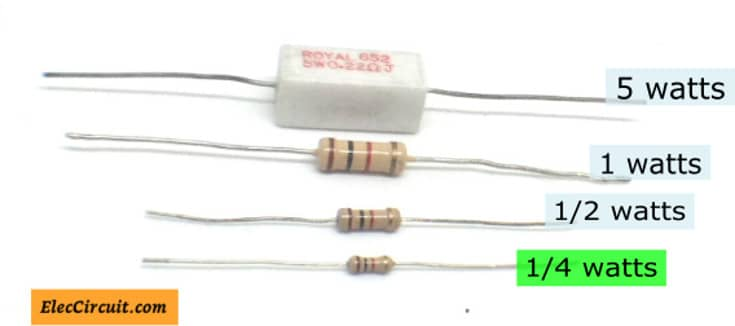
\includegraphics[width=0.72\textwidth]{figures/fig_resistors.jpg}
    \caption{Physical package comparison of resistors across various power ratings ($1/4\text{ W}$, $1/2\text{ W}$, $1\text{ W}$, and $5\text{ W}$ ceramic block) \cite{eleccircuit_components}.}
    \label{fig:resistors_power}
\end{figure}

\subsubsection{Schematic Symbols for Resistors}
In circuit schematics, resistors and their adjustable variants are depicted by standard symbols:

\begin{figure}[htbp]
    \centering
    \begin{tabular}{ccc}
        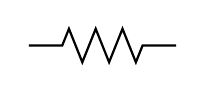
\begin{tikzpicture}[scale=0.85, baseline=-0.5ex]
            \draw[thick] (0,0) -- (0.5,0) -- (0.6,0.25) -- (0.8,-0.25) -- (1.0,0.25) -- (1.2,-0.25) -- (1.4,0.25) -- (1.6,-0.25) -- (1.7,0) -- (2.2,0);
        \end{tikzpicture}
        &
        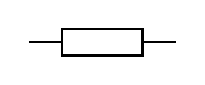
\begin{tikzpicture}[scale=0.85, baseline=-0.5ex]
            \draw[thick] (0,0) -- (0.5,0);
            \draw[thick, fill=white] (0.5,-0.2) rectangle (1.7,0.2);
            \draw[thick] (1.7,0) -- (2.2,0);
        \end{tikzpicture}
        &
        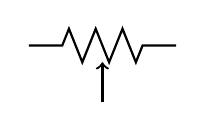
\begin{tikzpicture}[scale=0.85, baseline=-0.5ex]
            \draw[thick] (0,0) -- (0.5,0) -- (0.6,0.25) -- (0.8,-0.25) -- (1.0,0.25) -- (1.2,-0.25) -- (1.4,0.25) -- (1.6,-0.25) -- (1.7,0) -- (2.2,0);
            \draw[thick, ->] (1.1,-0.65) -- (1.1,-0.25);
            \draw[thick] (1.1,-0.65) -- (1.1,-0.85);
        \end{tikzpicture}
        \\
        \small \textbf{Fixed Resistor (US ANSI)} & \small \textbf{Fixed Resistor (IEC)} & \small \textbf{Potentiometer / Trimmer}
    \end{tabular}
    \caption{Standard schematic diagram symbols for fixed resistors and variable potentiometers.}
    \label{fig:resistor_symbols}
\end{figure}
\subsection{Capacitors}
Capacitors store electrical potential energy within an electrostatic field established between two conductive plates separated by an insulating dielectric medium. Capacitance is defined as:
\begin{equation}
    C = \frac{Q}{V}
\end{equation}
measured in Farads (F). In steady-state DC circuits, a charged capacitor behaves as an open circuit (blocking continuous DC current), while presenting low capacitive reactance ($X_C = \frac{1}{2\pi f C}$) to dynamic AC signals and transients.

\begin{figure}[htbp]
    \centering
    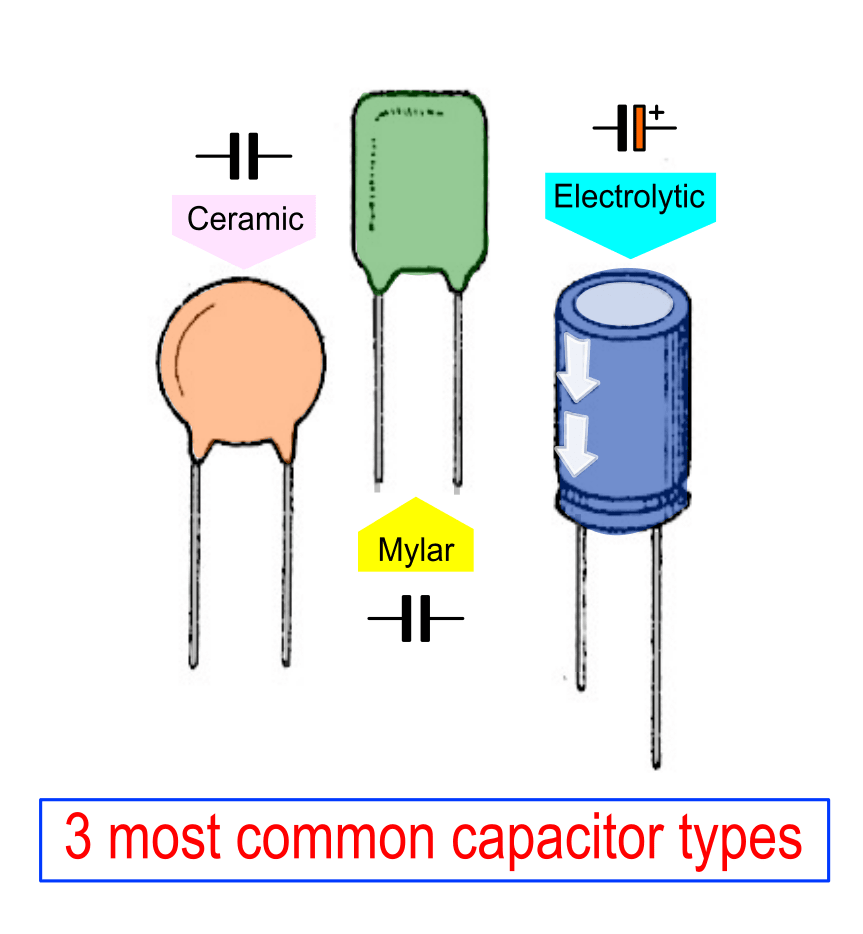
\includegraphics[width=0.72\textwidth]{figures/fig_capacitors.png}
    \caption{Three common capacitor types used in laboratory prototypes: Electrolytic, Ceramic, and Mylar \cite{eleccircuit_components}.}
    \label{fig:capacitors_types}
\end{figure}

\subsubsection{Capacitor Types, Polarity \& Marking Schemes}
\begin{itemize}[leftmargin=1.5em]
    \item \textbf{Electrolytic Capacitors (Polarized):} Feature high capacitance density ($0.1\ \mu\text{F}$ to $>10{,}000\ \mu\text{F}$). \textbf{Polarity is mandatory:} the negative lead is shorter and marked with a prominent white/gray stripe with minus signs ($-$). Connecting an electrolytic capacitor in reverse polarity can cause electrolyte boiling, gas venting, or catastrophic failure.
    \item \textbf{Ceramic and Mylar Capacitors (Non-Polarized):} Smaller capacitance values (picofarads to tenths of a microfarad) without polarity constraints.
    \item \textbf{3-Digit EIA Marking Code:} Non-polarized capacitors use a 3-digit numerical code in picofarads (pF):
    \begin{itemize}[leftmargin=1.2em]
        \item The first two digits represent the significant base value.
        \item The third digit represents the multiplier ($10^n$).
        \item \textit{Example:} A capacitor labeled \textbf{104} translates to $10 \times 10^4\text{ pF} = 100{,}000\text{ pF} = 0.1\ \mu\text{F}$.
    \end{itemize}
\end{itemize}

\subsubsection{Schematic Symbols for Capacitors}
\begin{figure}[htbp]
    \centering
    \begin{tabular}{ccc}
        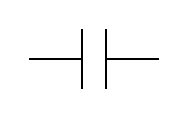
\begin{tikzpicture}[scale=0.85, baseline=-0.5ex]
            \draw[thick] (0,0) -- (0.8,0);
            \draw[thick] (0.8,0.45) -- (0.8,-0.45);
            \draw[thick] (1.15,0.45) -- (1.15,-0.45);
            \draw[thick] (1.15,0) -- (1.95,0);
        \end{tikzpicture}
        &
        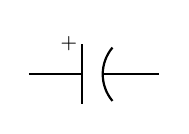
\begin{tikzpicture}[scale=0.85, baseline=-0.5ex]
            \draw[thick] (0,0) -- (0.8,0);
            \draw[thick] (0.8,0.45) -- (0.8,-0.45);
            \draw[thick] (1.25,0.4) arc (140:220:0.62);
            \draw[thick] (1.12,0) -- (1.95,0);
            \node[above, font=\scriptsize\bfseries] at (0.6,0.2) {$+$};
        \end{tikzpicture}
        &
        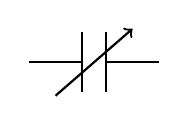
\begin{tikzpicture}[scale=0.85, baseline=-0.5ex]
            \draw[thick] (0,0) -- (0.8,0);
            \draw[thick] (0.8,0.45) -- (0.8,-0.45);
            \draw[thick] (1.15,0.45) -- (1.15,-0.45);
            \draw[thick] (1.15,0) -- (1.95,0);
            \draw[thick, ->] (0.4,-0.5) -- (1.55,0.5);
        \end{tikzpicture}
        \\
        \small \textbf{Non-Polarized Capacitor} & \small \textbf{Polarized (Electrolytic)} & \small \textbf{Variable Capacitor}
    \end{tabular}
    \caption{Standard schematic diagram symbols for non-polarized, polarized electrolytic, and variable capacitors.}
    \label{fig:capacitor_symbols}
\end{figure}
\subsection{Inductors \& Electromagnetic Energy Storage}
Inductors consist of insulated conductive wire wound into a helical coil around a magnetic core (ferrite, iron, or air). Inductors store energy within a concentrated magnetic field established by flowing current. The induced counter-electromotive force opposes instantaneous current fluctuations according to Faraday's and Lenz's laws:
\begin{equation}
    V = L \cdot \frac{di}{dt}
\end{equation}
where $L$ is inductance measured in Henries (H). Inductors resist abrupt changes in current, making them essential for switching regulator LC filters, choke suppression, and RF tuning networks.

\subsubsection{Schematic Symbols for Inductors}
\begin{figure}[htbp]
    \centering
    \begin{tabular}{ccc}
        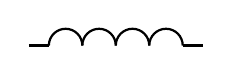
\begin{tikzpicture}[scale=0.85, baseline=-0.5ex]
            \draw[thick] (0,0) -- (0.3,0);
            \draw[thick] (0.3,0) arc (180:0:0.25);
            \draw[thick] (0.8,0) arc (180:0:0.25);
            \draw[thick] (1.3,0) arc (180:0:0.25);
            \draw[thick] (1.8,0) arc (180:0:0.25);
            \draw[thick] (2.3,0) -- (2.6,0);
        \end{tikzpicture}
        &
        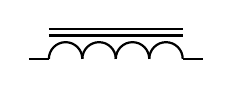
\begin{tikzpicture}[scale=0.85, baseline=-0.5ex]
            \draw[thick] (0,0) -- (0.3,0);
            \draw[thick] (0.3,0) arc (180:0:0.25);
            \draw[thick] (0.8,0) arc (180:0:0.25);
            \draw[thick] (1.3,0) arc (180:0:0.25);
            \draw[thick] (1.8,0) arc (180:0:0.25);
            \draw[thick] (2.3,0) -- (2.6,0);
            \draw[thick] (0.3,0.35) -- (2.3,0.35);
            \draw[thick] (0.3,0.45) -- (2.3,0.45);
        \end{tikzpicture}
        &
        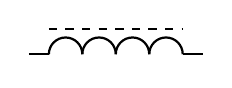
\begin{tikzpicture}[scale=0.85, baseline=-0.5ex]
            \draw[thick] (0,0) -- (0.3,0);
            \draw[thick] (0.3,0) arc (180:0:0.25);
            \draw[thick] (0.8,0) arc (180:0:0.25);
            \draw[thick] (1.3,0) arc (180:0:0.25);
            \draw[thick] (1.8,0) arc (180:0:0.25);
            \draw[thick] (2.3,0) -- (2.6,0);
            \draw[thick, dashed] (0.3,0.38) -- (2.3,0.38);
        \end{tikzpicture}
        \\
        \small \textbf{Air-Core Inductor} & \small \textbf{Iron-Core Inductor} & \small \textbf{Ferrite-Core Inductor}
    \end{tabular}
    \caption{Standard schematic diagram symbols for inductors with air, iron, and ferrite cores.}
    \label{fig:inductor_symbols}
\end{figure}
\section{Electrical Impedance and AC Circuit Dynamics}
While direct-current (DC) analysis evaluates circuits strictly through ohmic resistance ($R$), alternating-current (AC) signals introduce dynamic electromagnetic and electrostatic behaviors. The generalized opposition that an electrical network presents to the flow of sinusoidal alternating current is known as \textbf{electrical impedance} ($Z$).

Impedance is expressed mathematically as a complex number in rectangular and polar forms:
\begin{equation}
    Z = R + jX = |Z|\angle\theta
\end{equation}
where $j = \sqrt{-1}$ is the imaginary unit, and:
\begin{itemize}[leftmargin=1.5em]
    \item \textbf{Resistance ($R$):} The real part of impedance, measured in ohms ($\Omega$). It represents the irreversible dissipation of electrical energy into thermal heat ($P = I_{\text{rms}}^2 R$), occurring independently of signal frequency in ideal components.
    \item \textbf{Reactance ($X$):} The imaginary part of impedance, measured in ohms ($\Omega$). It represents the reversible storage and release of energy within electric fields (capacitive reactance, $X_C$) or magnetic fields (inductive reactance, $X_L$). Unlike resistance, reactance is strictly frequency-dependent.
    \item \textbf{Impedance Magnitude ($|Z|$):} The ratio of peak voltage to peak current:
    \begin{equation}
        |Z| = \sqrt{R^2 + X^2}
    \end{equation}
    \item \textbf{Phase Angle ($\theta$):} The temporal phase shift between voltage and current waveforms:
    \begin{equation}
        \theta = \arctan\left(\frac{X}{R}\right)
    \end{equation}
\end{itemize}

\subsection{Capacitive Reactance (\texorpdfstring{$X_C$}{X\_C})}
A capacitor opposes changes in voltage by accumulating electrostatic charge on its conductive plates. When subjected to a sinusoidal voltage with angular frequency $\omega = 2\pi f$, its complex impedance is given by:
\begin{equation}
    Z_C = \frac{1}{j\omega C} = -j\frac{1}{\omega C} = -j X_C
\end{equation}
where capacitive reactance is:
\begin{equation}
    X_C = \frac{1}{\omega C} = \frac{1}{2\pi f C}
\end{equation}
At zero frequency (DC, $f = 0$), $X_C \to \infty$, causing the capacitor to behave as an open circuit (blocking DC bias). As frequency increases, $X_C \to 0$, causing the capacitor to behave as an AC short circuit. This inverse frequency relationship forms the foundation of power supply decoupling, where capacitors shunt high-frequency transient noise to ground while preserving DC rails. In a pure capacitor, current leads voltage by $90^\circ$ ($\pi/2\text{ rad}$).

\subsection{Inductive Reactance (\texorpdfstring{$X_L$}{X\_L})}
An inductor opposes changes in current through the self-induction of counter-electromotive force (Lenz's Law). When driven by an alternating current, its complex impedance is:
\begin{equation}
    Z_L = j\omega L = +j X_L
\end{equation}
where inductive reactance is:
\begin{equation}
    X_L = \omega L = 2\pi f L
\end{equation}
At zero frequency (DC, $f = 0$), $X_L = 0\,\Omega$, allowing direct current to pass through with zero theoretical opposition. As frequency increases, $X_L$ scales linearly, presenting massive impedance to high-frequency AC signals. This direct frequency scaling allows inductors to function as electromagnetic interference (EMI) chokes and low-pass filtering elements. In a pure inductor, voltage leads current by $90^\circ$ ($\pi/2\text{ rad}$).

\subsection{Practical Engineering Applications of Impedance}
\begin{itemize}[leftmargin=1.5em]
    \item \textbf{Passive Frequency Filters:} Combining resistors with reactive elements produces frequency-selective networks, including RC/RL first-order low-pass filters (cut-off frequency $f_c = \frac{1}{2\pi RC}$) and high-pass filters used extensively in audio processing, sensor conditioning, and analog-to-digital converter (ADC) anti-aliasing.
    \item \textbf{Impedance Matching \& Signal Integrity:} In high-speed digital communications and RF systems, circuit traces behave as transmission lines. When the load impedance does not match the source and line characteristic impedance (typically $50\,\Omega$ in RF and $100\,\Omega$ differential in USB/Ethernet), signal reflections occur, generating ringing, false logic triggers, and severe data degradation.
\end{itemize}

\section{Active Semiconductor Devices}

\subsection{Diodes}
A semiconductor diode consists of a $p$-$n$ junction that acts as an electrical one-way valve for current flow. When forward-biased ($V > V_F$), current flows freely from \textbf{Anode ($A$)} to \textbf{Cathode ($K$)}. Under reverse bias, current flow is blocked.

\begin{figure}[htbp]
    \centering
    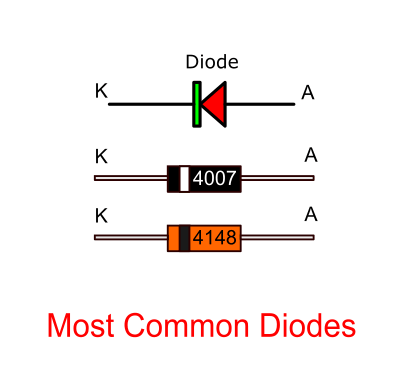
\includegraphics[width=0.68\textwidth]{figures/fig_diodes.png}
    \caption{Common semiconductor diodes (1N4007 power rectifier, 1N4148 high-speed signal) with physical cathode identification bands and corresponding schematic symbol \cite{eleccircuit_components}.}
    \label{fig:diodes_common}
\end{figure}

\subsubsection{Cathode Identification \& Types of Diodes}
\begin{itemize}[leftmargin=1.5em]
    \item \textbf{Cathode Marking Band:} On physical diode cylinders (such as the black epoxy 1N4007 or glass DO-35 1N4148), a painted silver or black band denotes the \textbf{Cathode ($K$)} terminal.
    \item \textbf{Zener Diodes:} Designed to operate in reverse breakdown at a stable, specified Zener voltage ($V_Z$), providing constant voltage regulation.
\end{itemize}

\begin{figure}[htbp]
    \centering
    \begin{tabular}{ccc}
        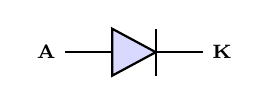
\begin{tikzpicture}[scale=0.85, baseline=-0.5ex]
            \draw[thick] (0,0) -- (0.7,0);
            \draw[thick, fill=blue!15] (0.7,0.35) -- (0.7,-0.35) -- (1.35,0) -- cycle;
            \draw[thick] (1.35,0.35) -- (1.35,-0.35);
            \draw[thick] (1.35,0) -- (2.05,0);
            \node[left, font=\scriptsize\bfseries] at (0,0) {A};
            \node[right, font=\scriptsize\bfseries] at (2.05,0) {K};
        \end{tikzpicture}
        &
        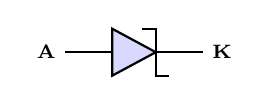
\begin{tikzpicture}[scale=0.85, baseline=-0.5ex]
            \draw[thick] (0,0) -- (0.7,0);
            \draw[thick, fill=blue!15] (0.7,0.35) -- (0.7,-0.35) -- (1.35,0) -- cycle;
            \draw[thick] (1.15,0.35) -- (1.35,0.35) -- (1.35,-0.35) -- (1.55,-0.35);
            \draw[thick] (1.35,0) -- (2.05,0);
            \node[left, font=\scriptsize\bfseries] at (0,0) {A};
            \node[right, font=\scriptsize\bfseries] at (2.05,0) {K};
        \end{tikzpicture}
        &
        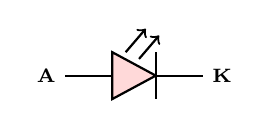
\begin{tikzpicture}[scale=0.85, baseline=-0.5ex]
            \draw[thick] (0,0) -- (0.7,0);
            \draw[thick, fill=red!15] (0.7,0.35) -- (0.7,-0.35) -- (1.35,0) -- cycle;
            \draw[thick] (1.35,0.35) -- (1.35,-0.35);
            \draw[thick] (1.35,0) -- (2.05,0);
            \draw[thick, ->] (0.9,0.35) -- (1.2,0.7);
            \draw[thick, ->] (1.1,0.25) -- (1.4,0.6);
            \node[left, font=\scriptsize\bfseries] at (0,0) {A};
            \node[right, font=\scriptsize\bfseries] at (2.05,0) {K};
        \end{tikzpicture}
        \\
        \small \textbf{Standard Diode} & \small \textbf{Zener Diode} & \small \textbf{Light Emitting Diode (LED)}
    \end{tabular}
    \caption{Schematic symbols for standard $p$-$n$ junction diodes, Zener voltage regulation diodes, and LEDs with emission rays.}
    \label{fig:diode_symbols}
\end{figure}
\subsection{Light Emitting Diodes (LEDs)}
Light Emitting Diodes (LEDs) are specialized $p$-$n$ junction diodes that emit light through electroluminescence when forward-biased. Because an unbuffered LED behaves as a near short-circuit once forward voltage threshold is exceeded, a series current-limiting resistor is mandatory.

\begin{figure}[htbp]
    \centering
    \begin{minipage}{0.48\textwidth}
        \centering
        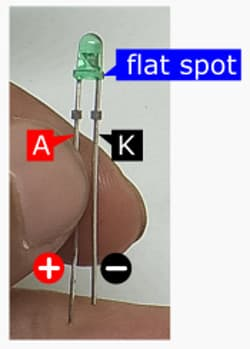
\includegraphics[width=\textwidth]{figures/fig_led_pinout.jpg}
        \caption{Physical pinout features of a standard LED: longer lead is Anode ($+$), shorter lead and flat rim spot indicate Cathode ($-$) \cite{eleccircuit_leds}.}
        \label{fig:led_pinout}
    \end{minipage}\hfill
    \begin{minipage}{0.48\textwidth}
        \centering
        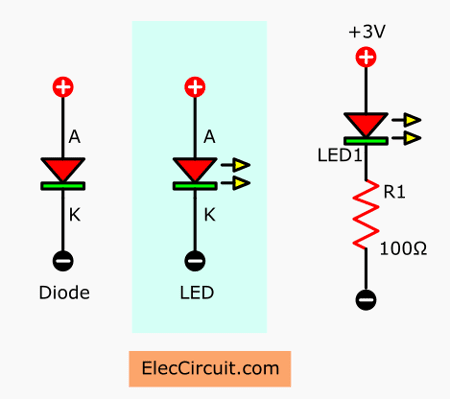
\includegraphics[width=\textwidth]{figures/fig_led_symbol.png}
        \caption{Schematic symbol of an LED showing current direction ($A \rightarrow K$) and outward radiation arrows \cite{eleccircuit_leds}.}
        \label{fig:led_symbol}
    \end{minipage}
\end{figure}

\subsubsection{LED Forward Voltages \& Polarity Rules}
\begin{itemize}[leftmargin=1.5em]
    \item \textbf{Polarity Verification:}
    \begin{itemize}[leftmargin=1.2em]
        \item \textbf{Lead Length:} The longer lead is the \textbf{Anode ($+$)}, and the shorter lead is the \textbf{Cathode ($-$/GND)}.
        \item \textbf{Flat Spot on Lens Rim:} When leads are trimmed, look for the flat edge molded onto the plastic lens perimeter; this always designates the \textbf{Cathode ($-$/K)}.
    \end{itemize}
    \item \textbf{Typical Forward Voltages ($V_F$):} Red ($\approx 1.7\text{ V}$), Yellow/Green ($\approx 2.1\text{--}2.3\text{ V}$), Blue/White ($\approx 3.3\text{--}3.6\text{ V}$).
\end{itemize}

\subsection{Transistors: BJT and MOSFET Architecture}
Transistors function as electronically controlled switches and current/voltage amplifiers:

\begin{figure}[htbp]
    \centering
    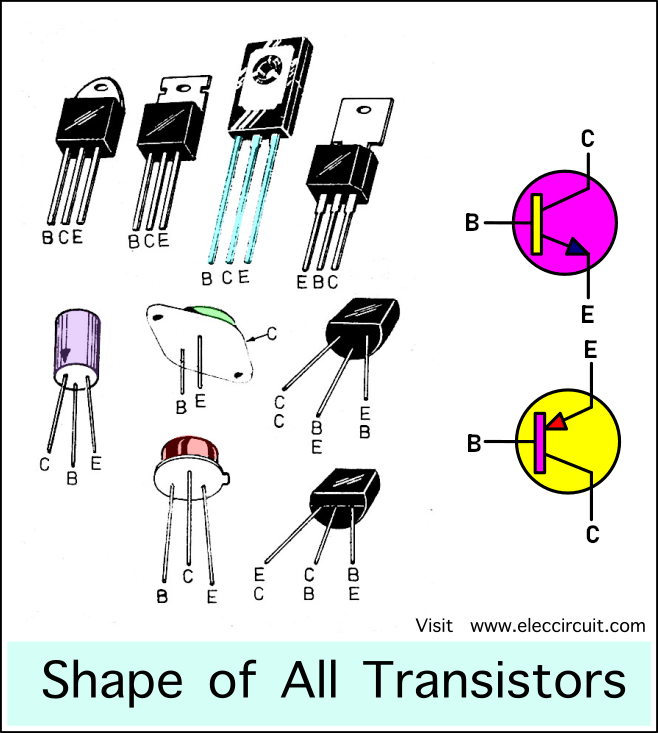
\includegraphics[width=0.75\textwidth]{figures/fig_transistor_shapes.png}
    \caption{Common physical transistor packages (TO-92, TO-220, TO-126) with terminal pinouts (B-C-E), and standard BJT schematic symbols (NPN vs. PNP) \cite{eleccircuit_components}.}
    \label{fig:transistor_shapes}
\end{figure}

\subsubsection{Bipolar Junction Transistors (BJTs)}
BJTs are 3-terminal, current-controlled devices comprising Base ($B$), Collector ($C$), and Emitter ($E$):
\begin{equation}
    I_C = \beta \cdot I_B
\end{equation}
where $\beta$ ($h_{FE}$) is the common-emitter forward current gain.
\begin{figure}[htbp]
    \centering
    \begin{tabular}{cc}
        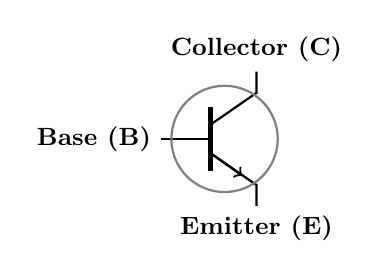
\begin{tikzpicture}[scale=0.9, baseline=-0.5ex]
            \draw[thick] (0,0) -- (0.7,0);
            \draw[ultra thick] (0.7,-0.45) -- (0.7,0.45);
            \draw[thick] (0.7,0.2) -- (1.35,0.65) -- (1.35,0.95);
            \draw[thick] (0.7,-0.2) -- (1.35,-0.65) -- (1.35,-0.95);
            \draw[thick, ->] (0.7,-0.2) -- (1.15,-0.52);
            \draw[thick, gray] (0.9,0) circle (0.75);
            \node[left, font=\small\bfseries] at (0,0) {Base (B)};
            \node[above, font=\small\bfseries] at (1.35,0.95) {Collector (C)};
            \node[below, font=\small\bfseries] at (1.35,-0.95) {Emitter (E)};
        \end{tikzpicture}
        &
        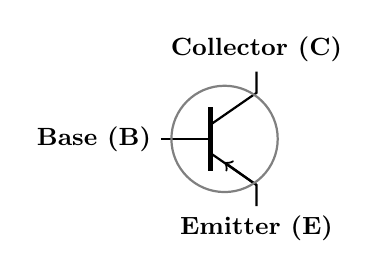
\begin{tikzpicture}[scale=0.9, baseline=-0.5ex]
            \draw[thick] (0,0) -- (0.7,0);
            \draw[ultra thick] (0.7,-0.45) -- (0.7,0.45);
            \draw[thick] (0.7,0.2) -- (1.35,0.65) -- (1.35,0.95);
            \draw[thick] (0.7,-0.2) -- (1.35,-0.65) -- (1.35,-0.95);
            \draw[thick, <-] (0.9,-0.33) -- (1.35,-0.65);
            \draw[thick, gray] (0.9,0) circle (0.75);
            \node[left, font=\small\bfseries] at (0,0) {Base (B)};
            \node[above, font=\small\bfseries] at (1.35,0.95) {Collector (C)};
            \node[below, font=\small\bfseries] at (1.35,-0.95) {Emitter (E)};
        \end{tikzpicture}
        \\
        \small \textbf{NPN BJT (Arrow Outward)} & \small \textbf{PNP BJT (Arrow Inward)}
    \end{tabular}
    \caption{Schematic symbols for NPN and PNP bipolar junction transistors, illustrating terminal designations and emitter current direction arrows.}
    \label{fig:bjt_symbols}
\end{figure}

\begin{itemize}[leftmargin=1.5em]
    \item \textbf{NPN Transistor:} Operates with positive collector voltage. The schematic symbol features an emitter arrow pointing \textbf{outward} (mnemonic: ``\textbf{N}ot \textbf{P}ointing i\textbf{N}'').
    \item \textbf{PNP Transistor:} Operates with negative collector bias. The schematic symbol features an emitter arrow pointing \textbf{inward} (mnemonic: ``\textbf{P}ointing i\textbf{N} \textbf{P}roudly'').
    \item \textbf{Terminal Pinouts:} Always verify package pinout specifications (e.g., E-B-C or B-C-E) because identical-looking TO-92 packages vary across transistor models.
\end{itemize}
\subsubsection{Field-Effect Transistors (MOSFETs)}
MOSFETs are voltage-controlled devices with near-infinite input impedance at DC. The voltage between Gate ($G$) and Source ($S$) creates an electric field modulating conductivity through the Drain ($D$) to Source channel.

\subsection{Integrated Circuits (ICs)}
Integrated Circuits (ICs) consolidate hundreds to millions of interconnected components onto a monolithic silicon die.

\begin{figure}[htbp]
    \centering
    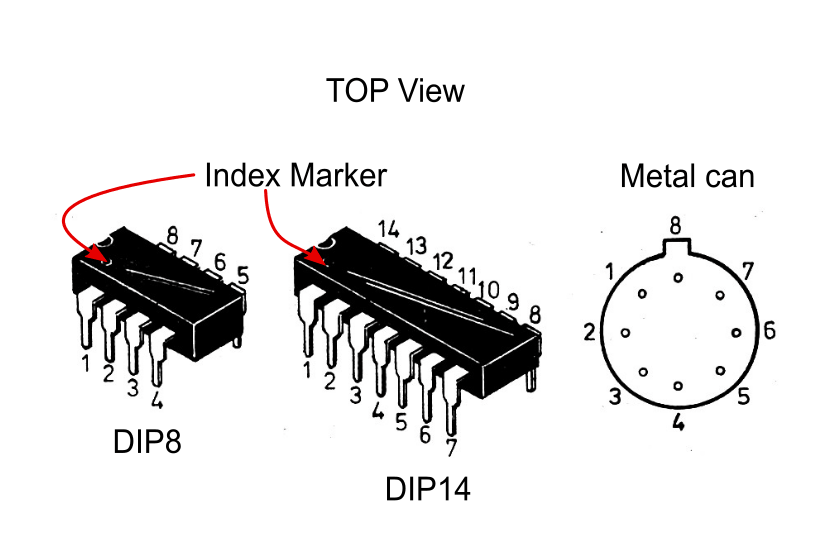
\includegraphics[width=0.75\textwidth]{figures/fig_ic_packages.png}
    \caption{Most common through-hole IC packages (DIP8, DIP14, and circular metal can) with index markers for pin numbering \cite{eleccircuit_components}.}
    \label{fig:ic_packages}
\end{figure}

\subsubsection{Pin Numbering Convention}
Through-hole Dual In-Line Packages (DIP8, DIP14, DIP16) follow a universal orientation standard:
\begin{enumerate}[leftmargin=1.5em]
    \item Locate the \textbf{index marker} (a semicircular notch or impressed dot) on the top face of the chip.
    \item Orient the notch facing to the left (or upward).
    \item Pin 1 is immediately to the left of the notch (or directly adjacent to the dot).
    \item Numbering increments \textbf{counter-clockwise} around the perimeter of the chip package, finishing at the top-left pin directly opposite Pin 1.
\end{enumerate}
\section{Series vs. Parallel Circuit Topologies}

\subsection{Series Circuits}
In a series topology, components are chained end-to-end along a single continuous path:
\begin{itemize}[leftmargin=1.5em]
    \item The current is identical through every component: $I_{total} = I_1 = I_2 = \dots = I_n$.
    \item Equivalent resistance is additive: $R_{eq} = \sum_{k=1}^n R_k$.
    \item Total voltage equals the sum of individual voltage drops (Kirchhoff's Voltage Law).
\end{itemize}

\subsection{Parallel Circuits}
In a parallel topology, components connect across two shared electrical nodes:
\begin{itemize}[leftmargin=1.5em]
    \item The voltage across every parallel branch is identical: $V_{total} = V_1 = V_2 = \dots = V_n$.
    \item Equivalent resistance is given by:
    \begin{equation}
        \frac{1}{R_{eq}} = \sum_{k=1}^n \frac{1}{R_k}
    \end{equation}
    \item Total current is the sum of branch currents (Kirchhoff's Current Law).
\end{itemize}

% !TEX root = ../main.tex
\chapter{Breadboard Prototyping \& Circuit Troubleshooting}

\section{Internal Architecture of Solderless Breadboards}
A solderless breadboard is an essential modular platform for rapid temporary circuit prototyping \cite{sparkfun_breadboard}. The internal architecture consists of molded thermoplastic housing enclosing spring-tempered phosphor bronze or nickel-silver clip strips:

\begin{enumerate}[leftmargin=1.5em]
    \item \textbf{Distribution Buses (Power Rails):} Longitudinal outer strips marked with red ($+$) and blue/black ($-$) color lines. These rails distribute DC supply voltage ($V_{CC}$) and system ground (GND) across the entire prototyping area.
    \item \textbf{Terminal Strips (Component Rows):} Arranged in vertical 5-hole tie-point groups. All 5 socket holes in a given column group are electrically bonded together by a common spring clip beneath the surface.
    \item \textbf{Central DIP Isolation Channel:} A $0.3\text{-inch}$ ($7.62\text{ mm}$) groove dividing the board halves. This channel matches standard Dual In-Line Package (DIP) IC lead spacing, ensuring opposing pins remain electrically isolated.
\end{enumerate}

\begin{figure}[htbp]
    \centering
    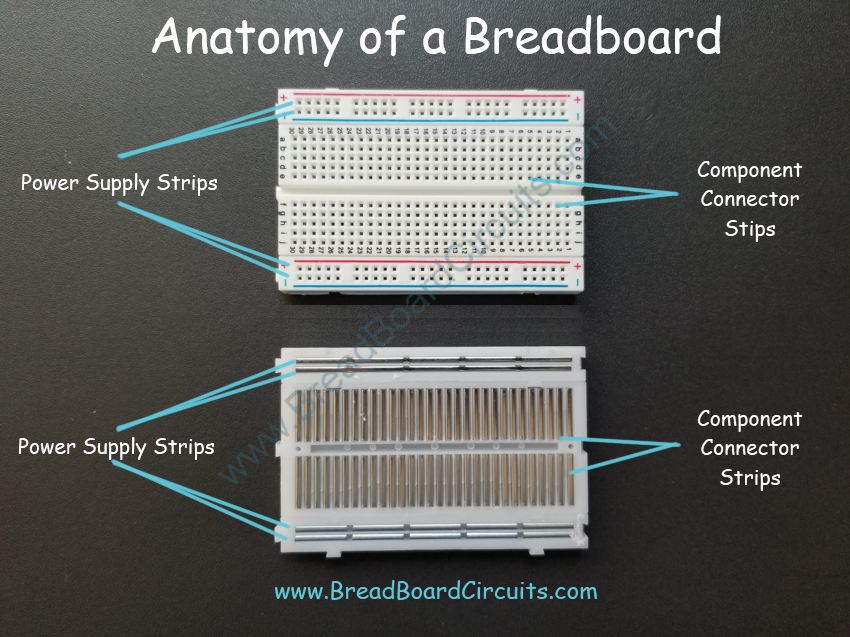
\includegraphics[width=0.78\textwidth]{figures/fig_breadboard_internal.jpg}
    \caption{Anatomy of a solderless breadboard showing the top face alongside the exposed reverse side, revealing the underlying metallic power distribution buses and vertical component terminal clip rows \cite{breadboardcircuits_anatomy}.}
    \label{fig:breadboard_internal}
\end{figure}

\section{Systematic Circuit Troubleshooting Methodology}
When an assembled prototype circuit fails to operate, technicians must avoid random component swapping. Systematic diagnostic methodology isolates the root cause rapidly:

\subsection{Step 1: Visual and Tactile Inspection (Power OFF)}
With power completely de-energized:
\begin{itemize}[leftmargin=1.5em]
    \item Verify semiconductor polarity: check LED anode/cathode orientation, electrolytic capacitor polarity bands, and diode cathode stripe bands.
    \item Inspect IC alignment: ensure the index notch/dot faces Pin 1 and no pins are folded or bent under the IC package.
    \item Check jumper seating: confirm wires are firmly seated in active terminal rows rather than loose or bridged across adjacent rows.
\end{itemize}

\subsection{Step 2: Static Power Supply Verification (Power ON)}
Energize the DC power supply:
\begin{itemize}[leftmargin=1.5em]
    \item Measure DC voltage directly at the breadboard power rail tie-points using a Digital Multimeter (DMM).
    \item Verify that rail voltage matches expected supply levels without excessive voltage drooping caused by power supply current limits or rail shorts.
\end{itemize}

\subsection{Step 3: Point-to-Point Node Voltage Tracing}
With circuit power active:
\begin{itemize}[leftmargin=1.5em]
    \item Secure the black DMM probe to system ground (GND).
    \item Progressively probe circuit nodes with the red DMM probe along the schematic signal path from source to load.
    \item Compare each measured DC node voltage against theoretical schematic calculations. A sudden divergence reveals open circuits, floating inputs, or defective components.
\end{itemize}

\subsection{Step 4: Resistance and Continuity Isolation (Power OFF)}
De-energize circuit power:
\begin{itemize}[leftmargin=1.5em]
    \item Set the DMM to audible continuity/resistance mode.
    \item Probe between nodes to verify low-resistance ($<1\ \Omega$) paths along expected traces and high-impedance ($>1\text{ M}\Omega$) isolation between adjacent, independent breadboard rows.
\end{itemize}

% !TEX root = ../main.tex
\chapter{Student Workshop Activity \& Worksheets}

\section{Activity 1: LED Indicator Breadboard Assembly \& Circuit Calculations}

\subsection{Objective \& Theoretical Parameter Calculations}
The objective of this laboratory exercise is to design, calculate, assemble, and quantitatively verify a current-limited LED indicator circuit on a solderless breadboard.

Given a regulated DC source voltage $V_{CC} = 5.0\text{ V}$, a standard indicator LED has a typical forward voltage drop $V_F \approx 2.0\text{ V}$ and a target forward current $I_F \approx 9.1\text{ mA}$ ($0.0091\text{ A}$). Applying Kirchhoff's Voltage Law (KVL) and Ohm's Law across the series loop:

\begin{equation}
    V_{CC} = V_R + V_F \implies V_R = V_{CC} - V_F
\end{equation}
\begin{equation}
    R = \frac{V_{CC} - V_F}{I_F} = \frac{5.0\text{ V} - 2.0\text{ V}}{0.0091\text{ A}} \approx 330\ \Omega
\end{equation}

Thus, a standard $330\ \Omega$ ($1/4\text{ W}$) resistor provides optimal current limiting, preventing thermal runaway and catastrophic semiconductor burnout.

\begin{figure}[htbp]
    \centering
    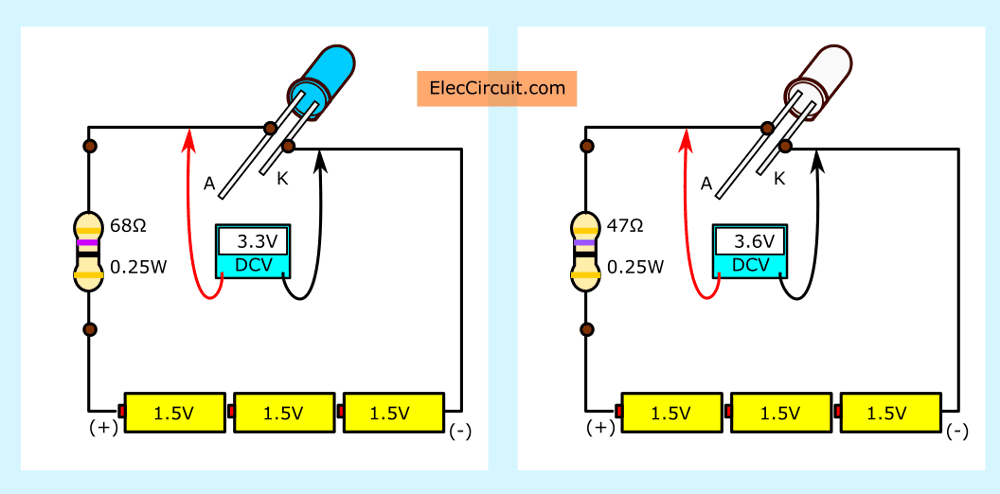
\includegraphics[width=0.88\textwidth]{figures/fig_led_schematic_wiring.png}
    \caption{Series LED indicator circuit schematic and Digital Multimeter (DMM) DC voltage probe verification across LED terminals ($A$ to $K$) using series current-limiting resistors \cite{eleccircuit_leds}.}
    \label{fig:led_schematic_wiring}
\end{figure}
\subsection{Step-by-Step Breadboard Assembly Protocol}
\begin{activitybox}
\textbf{ASSEMBLY PROTOCOL:}
\begin{enumerate}[leftmargin=1.5em]
    \item \textbf{Bench Power Configuration:} Turn on the DC power supply with output leads disconnected from the breadboard. Adjust the output to exactly $5.0\text{ V}$. Set the current limit knob to approximately mid-scale ($500\text{ mA}$). Turn the supply output switch OFF before connecting leads to the breadboard.
    \item \textbf{Rail Connections:} Connect the red power lead to the breadboard positive ($+$) bus and the black lead to the negative ($-$/GND) bus.
    \item \textbf{Resistor Placement:} Insert one lead of the $330\ \Omega$ resistor into the positive ($+$) rail and the other lead into terminal Row 10.
    \item \textbf{LED Insertion:} Identify the LED polarity: the longer lead is the \textbf{anode} ($+$) and the shorter lead with the flat cathode rim is the \textbf{cathode} ($-$). Insert the anode into terminal Row 10 (sharing the spring clip with the resistor) and the cathode into the negative ground rail.
    \item \textbf{Power Verification:} Energize the DC output. The LED will illuminate. Using a DMM set to DC Volts, verify approximately $5.0\text{ V}$ across the rails, $3.0\text{ V}$ across the resistor, and $2.0\text{ V}$ across the LED.
\end{enumerate}
\end{activitybox}

\section{Activity 2: Hands-On Demonstration --- Introduction to Soldering}

\subsection{Soldering Station Setup \& Temperature Calibration}
Soldering creates permanent electrical joints and mechanical bonds using an alloy filler metal.
\begin{itemize}[leftmargin=1.5em]
    \item \textbf{Personal Protective Equipment (PPE):} Safety glasses are mandatory. Ensure the local fume extractor is active.
    \item \textbf{Temperature Setting:} Set the soldering station to approximately \textbf{350\textdegree C (660\textdegree F)} for standard lead-free alloy solder wire. Allow 1--2 minutes for thermal equilibrium.
    \item \textbf{The Golden Rule:} Return the soldering iron to its safety stand the moment it leaves your hand. Never rest a hot iron on the bench surface.
\end{itemize}

\subsection{Tip Maintenance, Tinning, and Joint Formation}
\begin{enumerate}[leftmargin=1.5em]
    \item \textbf{Tip Cleaning \& Tinning:} Wipe the hot tip against a damp brass wire sponge or moist cellulose sponge. Immediately apply a small bead of fresh solder to the tip (tinning). This prevents oxidation and ensures rapid thermal conduction.
    \item \textbf{Heating the Joint:} Position the iron chisel tip so it makes simultaneous contact with both the copper PCB pad and the component lead. Hold for approximately 2 seconds to bring both surfaces up to soldering temperature.
    \item \textbf{Feeding Solder:} Introduce solder wire directly to the \textbf{heated joint} (not to the iron tip itself). The solder will melt, flow smoothly, and wet both surfaces.
    \item \textbf{Cooling:} Withdraw the solder wire first, followed immediately by the iron tip. Allow the joint to cool undisturbed for 3 seconds.
\end{enumerate}

\begin{figure}[htbp]
    \centering
    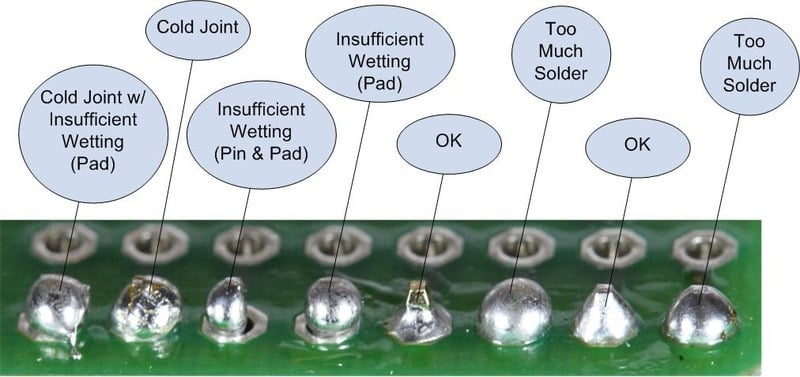
\includegraphics[width=0.88\textwidth]{figures/fig_solder_joints.jpg}
    \caption{Visual inspection criteria of PCB through-hole solder connections: distinguishing acceptable concave fillets (``OK'') from defective cold joints, insufficient pad/pin wetting, and excessive solder buildup \cite{adafruit_soldering_guide}.}
    \label{fig:solder_joints}
\end{figure}

\subsection{Joint Inspection Criteria}
\begin{itemize}[leftmargin=1.5em]
    \item \textbf{Acceptable Joint:} Features a shiny, smooth surface with a concave fillet (resembling a miniature tent or volcano) wetting both the lead and pad.
    \item \textbf{Defective Cold Joint:} Appears dull, grainy, or forms a spherical bead without wetting. To rework: reapply tip heat with a touch of flux-core solder for 2--3 seconds until reflow occurs.
    \item \textbf{Lead Trimming:} Trim excess component leads flush with the top of the solder fillet using flush wire cutters.
\end{itemize}

% !TEX root = ../main.tex
\chapter{Summary, Self-Assessment \& Next Steps}

\section{Key Takeaways Checklist}
Review the following learning checkpoints. Mark each box as you confirm your theoretical comprehension and practical laboratory competence:

\begin{itemize}[leftmargin=2em]
    \item[$\square$] \textbf{Laboratory Safety:} I recognize physiological shock thresholds ($1\text{ mA}$, $10\text{ mA}$, $20\text{--}30\text{ mA}$, $\ge 100\text{ mA}$), execute the ``One-Hand Rule'', understand ESD dissipation methods, and adhere to zero-hazard bench protocols.
    \item[$\square$] \textbf{Component Identification:} I can distinguish passive devices (resistors, capacitors, inductors) from active semiconductors (diodes, LEDs, BJTs, MOSFETs, and ICs) and interpret schematic symbols.
    \item[$\square$] \textbf{Breadboard Prototyping:} I understand the internal spring clip matrix, power bus rails, and center DIP isolation trench to assemble circuits accurately.
    \item[$\square$] \textbf{Systematic Troubleshooting:} I can perform a structured 4-step diagnostic protocol (visual inspection, rail voltage verification, node voltage tracing, and continuity checks) to isolate circuit faults.
    \item[$\square$] \textbf{Soldering Competence:} I can safely operate a soldering station at $350^\circ\text{C}$, tin tips, form concave fillets, and identify/remedy cold solder joints.
\end{itemize}

\section{Guided Reflection Questions}
Respond to the following technical review questions to reinforce core concepts:

\begin{enumerate}[leftmargin=1.8em]
    \item \textbf{Current-Limiting Resistor Function:} Why is a series resistor required when driving a semiconductor LED from an ideal voltage source, and what physical failure mode occurs if this resistor is omitted?
    \item \textbf{Breadboard Internal Topology:} Contrast the internal electrical continuity of the outer horizontal distribution buses against the inner vertical 5-hole terminal rows. How does this layout influence power routing?
    \item \textbf{Thermal Emergency Protocol:} What immediate sequence of actions must a technician take if a component on a prototype breadboard becomes excessively hot or begins to emit smoke during bench testing?
\end{enumerate}

\section{Next Steps \& Instructional Resources}
\begin{itemize}[leftmargin=1.5em]
    \item \textbf{Supplementary Reading:} Review assigned textbook readings on nodal circuit analysis and semiconductor physics.
    \item \textbf{Laboratory Review Quiz:} Complete the online post-workshop assessment module prior to the upcoming laboratory cycle.
    \item \textbf{Office Hours \& Technical Support:} For assistance with calculations, breadboard assemblies, or equipment operation, schedule consultation hours with laboratory instructors.
\end{itemize}


% ------------------------------------------------------------------------------
% References
% ------------------------------------------------------------------------------
\newpage
\bibliographystyle{IEEEtran}
\bibliography{references}

\end{document}
